\documentclass[border=4pt]{standalone}
\usepackage[utf8]{inputenc}
\usepackage[T1]{fontenc}
\usepackage{amsmath,amssymb}
\usepackage[table,gray]{xcolor}
\usepackage{tikz}
\usetikzlibrary{positioning,fit,calc,arrows.meta,shapes.geometric,decorations.pathreplacing,backgrounds}
\usepackage{pgfplots}
\pgfplotsset{compat=1.17}
\definecolor{stellantis}{RGB}{26,58,92}
\definecolor{sectionblue}{RGB}{44,95,138}
\definecolor{ddbrown}{RGB}{180,100,30}
\definecolor{ddbrownlight}{RGB}{255,243,230}
\begin{document}

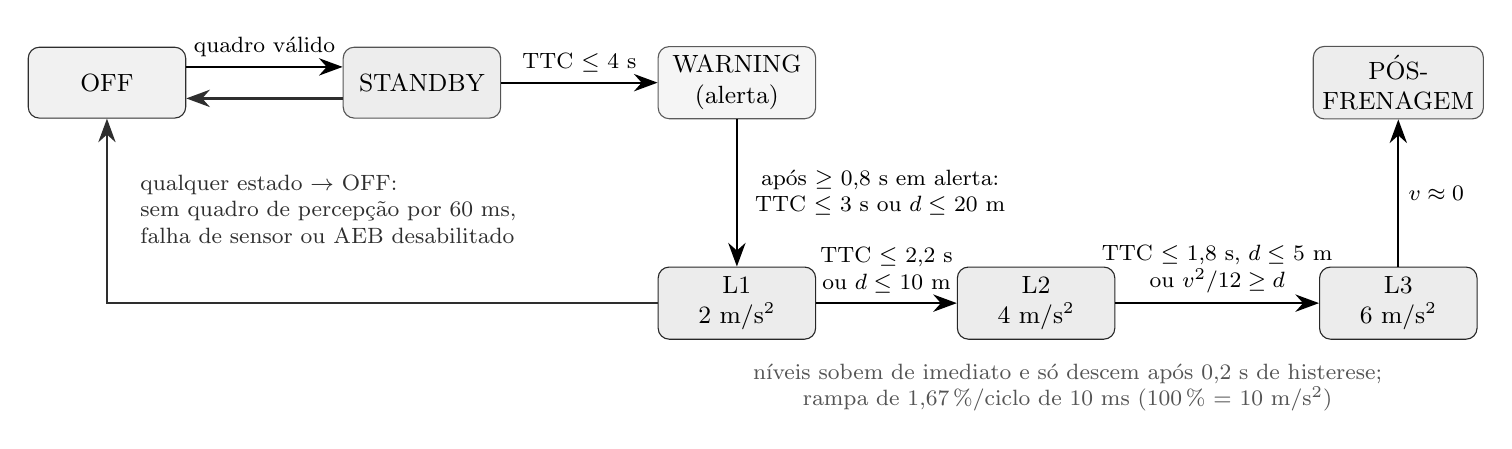
\begin{tikzpicture}[
    mod/.style={rectangle, draw, rounded corners=4pt, minimum height=1.0cm, font=\small, align=center, inner sep=4pt},
    int/.style={mod, fill=blue!8, draw=sectionblue},
    exec/.style={mod, fill=purple!10, draw=purple!60!black},
    ext/.style={mod, fill=gray!10, draw=gray!50},
    pert/.style={mod, fill=ddbrownlight, draw=ddbrown},
    ini/.style={mod, fill=green!8, draw=green!50!black},
    arr/.style={-{Stealth[length=3mm, width=2.2mm]}, thick},
    darr/.style={-{Stealth[length=2.5mm, width=2mm]}, thick, dashed, gray!70!black},
    lbl/.style={font=\footnotesize\ttfamily},
    nota/.style={font=\footnotesize, align=center},
    st/.style={rectangle, draw, rounded corners=4pt, minimum width=2.0cm, minimum height=0.9cm, font=\small, align=center},
    sb/.style={st, fill=blue!8, draw=sectionblue},
    sw/.style={st, fill=orange!10, draw=orange!60!black},
    so/.style={st, fill=red!8, draw=red!60!black},
    sl/.style={st, fill=purple!10, draw=purple!60!black},
    t/.style={font=\footnotesize, align=center},
]
% linha superior: estados sem frenagem; linha inferior: níveis de frenagem
\node[so] (off) at (0,0) {OFF};
\node[sb] (stb) at (4.0,0) {STANDBY};
\node[sw] (war) at (8.0,0) {WARNING\\(alerta)};
\node[sb] (pb) at (16.4,0) {PÓS-\\FRENAGEM};
\node[sl] (l1) at (8.0,-2.8) {L1\\2 m/s$^2$};
\node[sl] (l2) at (11.8,-2.8) {L2\\4 m/s$^2$};
\node[sl] (l3) at (16.4,-2.8) {L3\\6 m/s$^2$};
\draw[arr] (stb) -- node[t, above] {TTC $\le$ 4 s} (war);
\draw[arr] (war) -- node[t, right, xshift=1mm] {após $\ge$ 0{,}8 s em alerta:\\TTC $\le$ 3 s ou $d \le$ 20 m} (l1);
\draw[arr] (l1) -- node[t, above] {TTC $\le$ 2{,}2 s\\ou $d \le$ 10 m} (l2);
\draw[arr] (l2) -- node[t, above] {TTC $\le$ 1{,}8 s, $d\le$ 5 m\\ou $v^2/12 \ge d$} (l3);
\draw[arr] (l3) -- node[t, right] {$v \approx 0$} (pb);
\draw[arr] ([yshift=2mm]off.east) -- node[t, above] {quadro válido} ([yshift=2mm]stb.west);
\draw[arr, red!60!black] ([yshift=-2mm]stb.west) -- ([yshift=-2mm]off.east);
\draw[arr, red!60!black] (l1.west) -- (off.south |- l1.west) node[t, below, pos=0.5, xshift=4.0cm, red!60!black, align=center] {} -- (off.south);
\node[t, red!60!black, align=left, anchor=north west] at (0.3,-1.05)
   {qualquer estado $\to$ OFF:\\sem quadro de percepção por 60 ms,\\falha de sensor ou AEB desabilitado};
\node[t, sectionblue, align=center, anchor=north] at (12.2,-3.45)
   {níveis sobem de imediato e só descem após 0{,}2 s de histerese;\\rampa de 1{,}67\,\%/ciclo de 10 ms (100\,\% = 10 m/s$^2$)};
\end{tikzpicture}
\end{document}
